\documentclass[UTF8]{ctexart}
\ctexset{section = {format={\Large \bfseries}}}

\usepackage{lmodern}
\usepackage{amsmath}
\usepackage{graphicx}
\usepackage{float}
\usepackage{booktabs}
\usepackage{geometry}
\usepackage{listings}
\usepackage{xcolor}
\usepackage[ruled]{algorithm2e}


\geometry{a4paper,left=2cm,right=2cm,top=2cm,bottom=2cm}
% \lstset{
%     basicstyle=\tt,
%     %行号
%     numbers=left,
%     rulesepcolor=\color{red!20!green!20!blue!20},
%     escapeinside=``,
%     xleftmargin=2em,xrightmargin=2em, aboveskip=1em,
%     %背景框
%     framexleftmargin=1.5mm,
%     frame=shadowbox,
%     %背景色
%     backgroundcolor=\color[RGB]{245,245,244},
%     %样式
%     keywordstyle=\color{blue}\bfseries,
%     identifierstyle=\bf,
%     numberstyle=\color[RGB]{0,192,192},
%     commentstyle=\it\color[RGB]{96,96,96},
%     stringstyle=\rmfamily\slshape\color[RGB]{128,0,0},
%     %显示空格
%     showstringspaces=false
% }
%三线表表格模板
% \begin{table}[H]
%   \centering
%   \caption{\label{表i}\textbf{}}
%   \begin{tabular}{}
%   \toprule

%   \midrule

%   \bottomrule
% \end{tabular}
% \end{table}

%插入图片
% \begin{figure}[htbp]
%     \centering
%     \includegraphics[width=0.95\textwidth]{}
%     \caption{} 
% \end{figure}

% 列举
% \begin{itemize}
%   \item 
% \end{itemize}

\title{ \textbf{人工智能导论第二次作业问答题}}
\author{\textbf{祝尔乐}
        \textbf{2020013020}}
\date{\textbf{2022年4月28日}}
\begin{document}
\maketitle

\section{第一题}
\subsection*{(1)}
\noindent
正确。

\noindent
理由:
写出加入正则化的求解式的等价形式:
\begin{equation}
\hat{\textbf{w}} = \mathop{\arg \min}_{||\textbf{w}||_k \le r}
\sum_{i=1}^{n}(\textbf{w}^T \textbf{x}_i - y_i)^2, k=1,2
\end{equation}
\noindent
上式求出的解$w^*$可以看做由Lk范数(k=1,2)规定的半径为$r$的球面与
曲面$\sum_{i=1}^{n}(\textbf{w}^T \textbf{x}_i - y_i)^2 = Const$
的交点,相对于L2范数,L1范数与曲面的交点落在顶点的概率较大,
即交点更容易落在坐标轴上,于是得到的$w^*$较为稀疏。

\subsection*{(2)}
\noindent
错误。

\noindent
交叉验证中将用于训练的数据分为$k$折,然后循环的选取训练集和验证集
进行训练和验证,
而测试数据是不参与训练的,于是交叉验证中不需要使用测试数据。

\subsection*{(3)}
\noindent
错误。

\noindent
K邻近方法中K越小,模型的分类面越容易产生由噪声引起的畸变,变得不光滑。

\subsection*{(4)}
\noindent
错误。

\noindent
决策树也可以用于回归问题,例如最小二乘决策树。

\subsection*{(5)}
\noindent
错误。

\noindent
随机森林中,自举是相对于多次取样而言的,对基学习器而言,仍然是单次采样,
偏差不受自举影响,自举可以降低集成学习器的偏差。

\newpage
\section{第二题}
\noindent
消去$\xi$, 并令$\textbf{W}\leftarrow[\textbf{w}, b], \textbf{X}=[\textbf{x}, 1]$,
将问题形式转化为:
\begin{eqnarray}
        \mathop{\min}_{\textbf{W}} f(\textbf{W})\ while\ f(\textbf{W}) = 
        \frac{1}{2} || \textbf{W}||^2_2 + 
        \frac{C}{n} \sum_{i=1}^{n} 
        \gamma_i \max \{ 0, 1-y_i(\textbf{W}^T\textbf{X}_i)\}
\end{eqnarray}
\noindent
对上式求解次梯度:
\begin{equation}
        \bigtriangledown f = \frac{1}{2} \textbf{W} -
        \frac{C}{n} \sum_{i=1}^{n} 
        \gamma_i I[y_i(\textbf{W}^T\textbf{X}_i)<1]y_i\textbf{X}_i
\end{equation}
\noindent
使用梯度下降更新,设$\textbf{W}_t, Batch(t)$ 为$t$时刻的权值和训练样本的下标集,则:
\begin{eqnarray}
        \textbf{W}_{t+1} &=& \textbf{W}_t - \eta_t \bigtriangledown_t f\\
        &=& (1-\frac{1}{2}\eta_t )\textbf{W}_t + 
        \eta_t \frac{C}{n} \sum_{i \in Batch(t)} 
        \gamma_i I[y_i(\textbf{W}_t^T\textbf{X}_i)<1]y_i\textbf{X}_i
\end{eqnarray}
\noindent
写出算法伪代码:

\begin{algorithm*}[H]
        \caption{\texttt{SubGD-WeightSVM}($S, T, k$)}
        \KwIn{$S$(train set), $T$(max iteration num), $k$(batch num)}
        \KwOut{a approximation of $\textbf{W}$}
        Initialize $\textbf{W} $ with $ \textbf{0}$\\
        \For {$t \leftarrow 1$ $\mathbf{to}$ $T $}
        {
        Choose a random batch of size $k$ from $S$ as $A$(index)\\
        $A^+ \leftarrow \{i \in A :y_i(\textbf{W}_i^T \textbf{X}_i) < 1\}$\\
        $\eta \leftarrow \frac{2}{t}$\\
        $\textbf{W} \leftarrow (1-\frac{1}{2}\eta )\textbf{W} - \eta \frac{C}{k} \sum_{i \in A^+} \gamma_i y_i\textbf{X}_i$
        }
        \Return{$\textbf{W}$}
\end{algorithm*}

% \begin{algorithm}[H]
%     \renewcommand{\thealgocf}{}
%     \caption{\texttt{SA-solve-k-Knights}($problem, schedule$)}
%     \KwIn{problem, schedule}
%     \KwOut{a solution state}
%     $current \leftarrow problem.INITIAL$\\
%     \For {$t \leftarrow 1$ $\mathbf{to}$ $\infty $}
%     {
%         $ T \leftarrow schedule(t)$\\
%         \If(){$T = 0$}{
%             \textbf{return} $current$
%         }

%         $ next \leftarrow  $a random successor of $current$\\

%         $\Delta E \leftarrow VALUE(current) - VALUE(next)$\\
%         \If(){$\Delta E > 0$}
%         {
%             $current \leftarrow next$
%         }
%         \Else(){
%             with probability $e^{\frac{\Delta E}{kT}}$ : $current \leftarrow next$
%         }


%     }
% \end{algorithm}
\newpage
\section{第三题}
推导如下:
%插入图片
\begin{figure}[htbp]
    \centering
    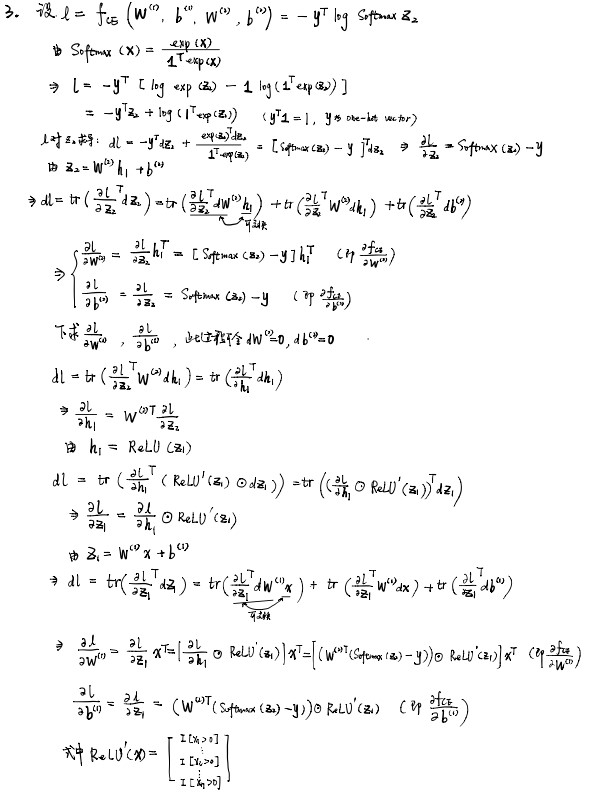
\includegraphics[width=0.85\textwidth]{images/Q3.jpg}
\end{figure}

\section{第四题}
在classification文件夹中。

\end{document}

